\documentclass{report}
% Comment the following line to NOT allow the usage of umlauts
\usepackage[utf8]{inputenc}
% Uncomment the following line to allow the usage of graphics (.png, .jpg)
\usepackage{geometry}
\geometry{left=3cm,right=3cm,top=3cm,bottom=3cm}

\usepackage[usenames,dvipsnames]{color}
\usepackage[colorlinks,linkcolor=NavyBlue,anchorcolor=red,citecolor=green]{hyperref}
\usepackage{graphicx}
\usepackage{enumerate}
\usepackage{multirow}
\usepackage{float}
\usepackage{bm}
\usepackage{array,makecell}
\usepackage[table,xcdraw]{xcolor}

\usepackage{amsmath,amsfonts}
%\usepackage[utopia]{mathdesign}
\usepackage[charter]{mathdesign}
%\usepackage{unicode-math}
%\setmathfont{Latin Modern Math}
%\setmathfont{TG Termes Math}

\usepackage[thmmarks,amsmath]{ntheorem}
\usepackage{tikz}
\theorembodyfont{\upshape}
\newtheorem{definition}{Definition}[section]
\newtheorem{example}{Example}[section]
\newtheorem{proposition}{Proposition}[section]
\newtheorem{theorem}{Theorem}[section]
\newtheorem{lemma}{Lemma}[section]
\theoremstyle{nonumberplain}
\theoremheaderfont{\itshape}
\theorembodyfont{\normalfont}
\theoremsymbol{\\ \rightline{$\square$}}
\newtheorem{proof}{Proof.}

\newcommand{\E}{\mathrm{E}}
\newcommand{\Var}{\mathrm{Var}}
\newcommand{\Cov}{\mathrm{Cov}}
\newcommand{\y}{\mathbf{y}}
\newcommand{\Y}{\mathbf{Y}}
\newcommand{\X}{\mathbf{X}} 
\newcommand{\M}{\mathbf{M}} 
\newcommand{\e}{\mathbf{e}} 
\newcommand{\0}{\mathbf{0}} 
\newcommand{\vbe}{\bm{\beta}}   
\newcommand{\vep}{\bm{\varepsilon}}  
\newcommand{\vb}{\mathbf{b}} 

% Start the document
\begin{document}
	\begin{center}	
	~\\ 
	\vspace{6em} 
	\textsc{\Huge Machine Learning}	
	~\\
	\vspace{2.5em} 
	{\Large From the Perspective of Statistics}
	~\\
	\vspace{6em}
	\textsf{Huyi Chen}
	~\\
	\vspace{5in}  
	{\large Latest Update: \today}
	\end{center}

% Create a new 1st level heading
\chapter{Introduction}

\section{Terminology and Framework}

\begin{itemize}
	\item \textbf{Data generating process}: $X$ is a $p-\text{dimensional}$ random vector with joint distribution $\mathrm{P}(x)$ and $Y=f(X)$ is a random variable.
	\begin{itemize}
		\item Input vector: $X\in D\subset\mathbb{R}^p$.
		\item Output vector: $Y\in G\subset\mathbb{R}$.
		\item Data: Given the sample $S=\{(X_1,Y_1),(X_2,Y_2),\cdots,(X_{N+M},Y_{N+M})\}$ where $(X_1,X_2,\cdots,X_{N+M})$ follows the distribution $\mathrm{P}(x)$, both the training data $T=\{(x_1,y_1),(x_2,y_2),\cdots,(x_{N},y_{N})\}$ and text data $Q=\{(x_{N+1},y_{N+1}),(x_{N+2},y_{N+2}),\cdots,(x_{N+M},y_{N+M})\}$ consist of the realization values of the sample.
	\end{itemize}	

	Considering that in general $Y$ cannot be totally determined by $X$, the data generating process of the learning model can be extended: $(X,Y)$ is a $(p+1)-\text{dimensional}$ random vector with joint distribution $\mathrm{P}(x,y)$.
	\begin{itemize}
		\item Input vector: $X\in D\subset\mathbb{R}^p$.
		\item Output vector: $Y\in G\subset\mathbb{R}$.
		\item Data: Given the sample $S=\{(X_1,Y_1),(X_2,Y_2),\cdots,(X_{N+M},Y_{N+M})\}$ following the distribution $\mathrm{P}(x,y)$, both the training data $T$ and text data $Q$ consist of the realization values of the sample.
	\end{itemize}

	\item \textbf{Objective}: Given the sample $S$, estimate a decision function $\hat{f}\in\mathcal{F}$ trying to minimize the expected prediction error (EPE)
	\[
	\mathrm{E}[L(Y,f(X))].
	\]
	\begin{itemize}
		\item Decision function: $f:\mathbb{R}^p\supset D\to\mathbb{R},x\mapsto f(x)$ serves to produce the prediction of $Y$, provided a specified value $x$ of $X$. 
		\item Loss function: $L(Y,f(X))$ normally has the form of 
		\[
		L_2=(Y-f(X))^2\ \text{ or }\ L_1=|Y-f(X)|\ \text{ or }\ L_I=1_{Y\ne f(X)}.
		\]
		\item Hypothesis space: $\mathcal{F}$ is a collection of all potential decision functions $f$ to be selected. In some cases, we suppose that $f$ as a candidate can be specified by several parameters. Thus $\mathcal{F}=\{f_\theta|Y=f_\theta(X),\;\theta\in\mathbb{R}^n\}$ can be described by the parametric space $\Theta=\{\theta:Y=f_\theta(X),\;\theta\in\mathbb{R}^n\}$.
	\end{itemize}
	If the probability distribution of $(X,Y)$ was known to us, it might succeed to find the optimal solution $\tilde{f}$ of the following minimization problem
	\[
	\min_{f\in\mathcal{F}}\mathrm{E}[L(Y,f(X))]
	\]
	in virtue of the optimization theory. In other words, what need to be settled is purely an optimization problem rather than a statistical problem. Unfortunately, the specific distribution of $(X,Y)$ is inaccessible in reality. Thus we can only exploit the training data to estimate an acceptable decision function $\hat{f}$, with acceptance of the fact that $\hat{f}$ in general has a greater EPE than $\tilde{f}$. 
	
	\item \textbf{Optimization strategies}: Since the EPE minimization problem is ill-formed, we have developed two major strategies to produce a tractable optimization problem. 
	\begin{itemize}
		\item Empirical risk minimization: according to the law of large numbers, if some regular conditions$\footnote{For example, the uniform law of large numbers can be applied here. The details are consigned to the appendix}$ hold, then as $N\to\infty$, the solution of the following minimization problem will converge to the theoretically optimal solution $\tilde{f}$.
		\[
		\min_{f\in\mathcal{F}}\frac{1}{N}\sum_{i=1}^{N}L(Y_i,f(X_i))
		\]
		
		\item Structural risk minimization: In reality, the size of training set $N$ is limited and accordingly the method of empirical risk minimization may not generate a function $\hat{f}$ which is sufficiently close to $\tilde{f}$. Later we will elaborate this phenomenon named "overfitting". However, if we add a regularizer or penalty term $\lambda J(f)$ to penalize the complexity of the decision function $f$ as follows
		\[
		\min_{f\in\mathcal{F}}\frac{1}{N}\sum_{i=1}^{N}L(Y_i,f(X_i))+\lambda J(f),
		\]
		it is possible to lead to a better result.
	\end{itemize} 
\end{itemize} 



		
	
\section{The Common Form of Optimal Decision Function }
\subsection{Loss function for quantitative output variables: squared error loss}
Let $Y\in\mathbb{R}$ be a quantitative variable. And we take the most
common and convenient loss function, squared error loss
\[
L(Y,f(X))=(Y-f(X))^2.
\]
In this case, the problem of minimizing the expected prediction error becomes
\[
\min_{f\in\mathcal{F}}\mathrm{E}[(Y-f(X))^2]=\min_{f\in\mathcal{F}}\int (y-f(x))^2\;\mathrm{dP}(x,y).
\]
Note that
\[\mathrm{E}[(Y-f(X))^2]=\mathrm{E}[\mathrm{E}[(Y-f(X))^2|\; X]]=\int\mathrm{E}[(Y-f(x))^2|\; X=x]\;\mathrm{dP}(x).\]
It suffices to minimize EPE pointwise, that is, 
\begin{align*}
&\ \ \min_{f(x)\in\mathbb{R}}\mathrm{E}[(Y-f(x))^2|\; X=x]\\
&=\min_{c\in\mathbb{R}}\mathrm{E}[(Y-c)^2|\; X=x]\\
&=\min_{c\in\mathbb{R}}\mathrm{Var}[Y-c|\; X=x]+(\mathrm{E}[(Y-c)|\; X=x])^2\\
&=\min_{c\in\mathbb{R}}\mathrm{Var}[Y|\; X=x]+(\mathrm{E}[Y|\; X=x]-c)^2.\\
\end{align*}
We see the optimal solution is
\[
\tilde{f}(x) = \mathrm{E}[Y|\; X=x],
\]
Thus the best prediction of $Y$ at any point $X = x$ is the conditional expectation, when best is measured by average squared error. \\
Later in this book we are to develop effective methods to estimate the conditional expectation $\mathrm{E}[Y|\; X=x]$.
\subsection{Loss function for categorical output variable: 0-1 indicator}
Assume that $Y\in G$ is a categorical variable and that the set of possible classes is $G=\{G_1,G_2,\cdots,G_K\}$. This time the 0–1 loss function 
\[
L(Y,f(X))=1_{Y\ne f(X)}=
\begin{cases}
0,&Y=f(X),\\
1,&Y\ne f(X),
\end{cases}
\]
is adopted for simplification. Likewise it suffices to minimize EPE pointwise.
\begin{align*}
&\ \ \min_{f(x)\in G}\mathrm{E}[1_{Y\ne f(x)}|\; X=x]\\
&=\min_{g\in G}\mathrm{E}[1-1_{Y=g}|\; X=x]\\
&=\min_{g\in G}1-\mathrm{P}(Y=g|\; X=x)
\end{align*}
And the optimal solution is
\[
\tilde{f}(x)=\max_{g\in G} \mathrm{P}(Y=g|\; X=x)
\]

\section{Generalization Error Bound}

As is mentioned before, we always hope that $\hat{f}$ has as small EPE as possible. EPE is also called the generalization error, indicating it gauges the performance of the selected function $\hat{f}$ in a general sense. We also emphasize that without knowing the probability distribution of $(X,Y)$, there is no way to calculate the expectation of $L(Y,f(X))$. In practice, it is typical to analyze the upper bound of generalization error to describe the generalization ability of the selected function $\hat{f}$. 

In the case of binary classifications, deriving the generalization error bound is relatively simple. Let's denote the generalization error and the empirical error by
\begin{align*}
	R(f)=\mathrm{E}[L(Y,f(X))]
\end{align*}
and
\[
\hat{R}(f)=\frac{1}{N} \sum_{i=1}^{N} L\left(Y_{i}, f\left(X_{i}\right)\right),
\]
respectively. Actually, We have the following result.

\begin{theorem}
	Suppose that the training set $T=\{(X_1,Y_1),(X_2,Y_2),\cdots,(X_{N},Y_{N})\}$ with $X_i\in\mathbb{R}^p$ and $Y_i\in\{+1,-1\}$ is generated from the distribution $\mathrm{P}(x,y)$. If the hypothesis space is a finite set $\mathcal{F}=\{f_1,f_2,\cdots,f_d\}$, then for any $f\in \mathcal{F}$, with a probability of not less than $1-\delta$ we have
	\[
	R(f) \le \hat{R}(f)+\varepsilon(d, N, \delta)
	\]
	where 
	\[
	\varepsilon(d, N, \delta)=\sqrt{\frac{1}{2 N}\left(\log d+\log \frac{1}{\delta}\right)}.
	\]
\end{theorem}









\chapter{Linear Model}
\section{Finite Sample Linear Model}
\subsection{Statistic model setup}
Linear model supposes the data generating process is
\[
Y= X^T\beta+\varepsilon,
\]
where $X=(1,X^{(1)},\cdots,X^{(p)})\in\mathbb{R}^{p+1}$, $Y\in\mathbb{R}$, $\beta\in\mathbb{R}^{p+1}$ is an unknown parameter and $\varepsilon$ is an error term which cannot be directly observed. Without loss of generality, we can always assume that $\E[\varepsilon|\;X]=0$.
Given a finite sample $(\X,\y)$ of size $n$, the linear Model indicates 
\[
\Y = \X \beta +\vep,
\]
where
\[
\Y=
\begin{pmatrix}
Y_1\\
Y_2\\
\vdots\\
Y_N
\end{pmatrix}
,\;\X=
\begin{pmatrix}
1& x_{11}&\cdots& x_{1p}\\
1& x_{21}&\cdots &x_{2p}\\
\vdots&\vdots& &\vdots\\
1& x_{N1}&\cdots &x_{Np}
\end{pmatrix}
\renewcommand*{\arraystretch}{1.5}
=\begin{pmatrix}
X_1^T\\
X_2^T\\
\vdots\\
X_N^T
\end{pmatrix}
\renewcommand*{\arraystretch}{1}
,\;
\beta=
\begin{pmatrix}
\beta_0\\
\beta_1\\
\vdots\\
\beta_p
\end{pmatrix}
,\;
\vep=
\begin{pmatrix}
\varepsilon_1\\
\varepsilon_2\\
\vdots\\
\varepsilon_N
\end{pmatrix}.
\]
\subsection{Ordinary least square estimate}
If we take squared error loss, then the best prediction of $Y$ is
\[
\tilde{f}(X) = \mathrm{E}[Y|\; X]=X'\beta.
\]
We can use least square method to estimate the parameter $\beta$ in the linear model, by minimizing the residual sum-of-squares
\[
\hat{\beta}=\arg\min_{\theta\in\mathbb{R}^{p+1}}\, RSS(\theta)=\arg\min_{\theta\in\mathbb{R}^{p+1}}\sum_{i=1}^N(Y_i-X_i^T\theta)^2.
\]
If $\X$ is of full column rank, the optimization problem has a unique solution
\[
\hat{\beta}=(\X^T\X)^{-1}\X^T\Y.
\]
The statistic properties of the OLS estimator $\hat{\beta}$ is remarkable. According to Gauss-Markov theorem, Under Assumptions 1.1-1.4
\begin{enumerate}
	\item[1.1]linearity:\quad $Y_i= X_i^T\beta+\varepsilon_i$, $(i=1,2,\cdots,N)$,
	\item[1.2] strict exogeneity:\quad $\E[\vep|\;\X]=0$,
	\item[1.3] no multicollinearity:\quad  $\mathrm{P}(\mathrm{rank}(\X)=p+1)=1$,
	\item[1.4] spherical error variance:\quad $\Var[\vep|\;\X]=\sigma^2>0$,
\end{enumerate}
$\hat{\beta}$ is the best linear unbiased estimator(BLUE). That is, for any unbiased estimator $\hat{\theta}$ that is linear in $\Y$, 
\[
\Var[\hat{\theta}|\;\X]\ge\Var[\hat{\beta}|\;\X]
\]
in the matrix sense. 

\chapter{SVM}

\section{linear SVM}

\begin{align*}
	\max _{\beta, \beta_{0},\|\beta\|=1} &M\\
	\text { subject to } y_{i}\left(x_{i}^{T} \beta+\beta_{0}\right)& \geq M, i=1, \ldots, N
\end{align*}




\chapter{KNN}

\section{Nearest-neighbor methods}
Nearest-neighbor methods use those observations in the training set $T$ closest in input space to $x$ to estimate the aforementioned conditional expectation  $\mathrm{E}[Y|\; X=x]$. Specifically, the $k$-nearest neighbor fit for $\hat{Y}$ is defined as follows:
\begin{itemize}
	\item Quantitative output
	\[
	\hat{Y}=\hat{f}(x)=\dfrac{1}{k}\sum_{i:x_i\in N_k(x)}y_i,
	\]
	\item Categorical output
	\[
	\hat{Y}=\hat{f}(x)=\arg\max_{g\in G}\sum_{i:x_i\in N_k(x)}1_{y_i=g},
	\]
\end{itemize}
where $N_k(x)$ is the neighborhood of $x$ defined by the $k$ closest points $x_i$ in the training sample. Closeness implies a metric, which for the moment we assume is Euclidean distance 
\[
\Vert x_1-x_2\Vert_2=(x_1-x_2)^2.
\].


\chapter{Decision Tree}
Tree-based methods partition the feature space into a set of rectangles, and
then fit a simple model (like a constant) in each one. We first describe a popular tree-based method called CART (classification and regression tree), and later contrast it with C4.5, a major competitor. CART requires a specific hypothesis space $\mathcal{F}$ which consists of functions of such forms:
\[
f(x)=\sum_{m=1}^{M} c_{m} 1\left[x \in R_{m}\right],
\]
where $p$-dimensional rectangular regions $R_1,R_2,\cdots,R_M$ constitute a recursive partition of the feature space $\mathbb{R}^p$. That is, if a partition $P_J=(R_1,R_2,\cdots,R_J)$ has been obtained, we just cut some rectangular region $R_m(1\le m\le J)$ into two parts by a $p-1$-dimensional hyperplane $x^{(i)}=\ell_J(1\le i\le p)$ to produce a new partition $P_{J+1}=(R'_1,R'_2,\cdots,R'_{J+1})$
\section{Regression Trees}
Assume the output $Y$ is a continuous variable. Then it leads to the concept of regression trees. Conventionally we choose the squared error loss and accordingly obtain the minimization problem
\begin{align*}
\min_{f\in\mathcal{F}}\mathrm{E}[(Y-f(X))^2]&=\min_{f\in\mathcal{F}}\mathrm{E}\left[\left(\sum_{m=1}^{M} (Y-c_{m}) 1_{X \in R_{m}}\right)^2\right]\\
&=\min_{f\in\mathcal{F}}\mathrm{E}\left[\sum_{m=1}^{M} (Y-c_{m})^2 1_{X \in R_{m}}\right]\\
&=\min_{f\in\mathcal{F}}\int\mathrm{E}\left[\left.\sum_{m=1}^{M} (Y-c_{m})^2 1_{x \in R_{m}}\right|X=x\right]\mathrm{dP}(x)\\
&=\min_{f\in\mathcal{F}}\sum_{m=1}^{M}\int_{ R_{m}}\mathrm{E}\left[\left. (Y-c_{m})^2\right|X=x\right]\mathrm{dP}(x).
\end{align*}
It is easy to see whichever partition is specified, the optimal $c_m$ remains
\[
\tilde{c}_m = \mathrm{E}[Y|\; X\in R_{m}].
\]
Now let's consider the empirical risk minimization problem
\[
\min_{f\in\mathcal{F}}\frac{1}{N}\sum_{i=1}^{N}L(Y_i,f(X_i))=\min_{f\in\mathcal{F}}\frac{1}{N}\sum_{i=1}^{N}\sum_{m=1}^{M} (Y_i-c_{m})^2 1_{X_i \in R_{m}}.
\]
Thus the proper estimate of $\hat{c}_m$ is just the average of $Y_i$ in region $R_{m}$
\[
\hat{c}_{m}=\operatorname{ave}\left(Y_{i} | X_{i} \in R_{m}\right).
\]
However, finding the best binary partition in terms of minimum sum of squares
is generally computationally infeasible. Hence we proceed with a greedy
algorithm. Starting with all of the data, consider a splitting variable indexed by $r\in\{1,2,\cdots,p\}$ and
split point $s\in\mathbb{R}$, and define the pair of half-planes
\[
R_{1}(r, s)=\left\{X\in\mathbb{R}^p | X^{(r)} \leq s\right\} \text { and } R_{2}(r, s)=\left\{X\in\mathbb{R}^p  | X^{(r)}>s\right\}.
\]
Then we seek the splitting variable $r$ and split point $s$ that solve
\begin{align*}
&\min _{r, s}\left[\min _{c_{1}} \sum_{X_{i} \in R_{1}(r, s)}\left(Y_{i}-c_{1}\right)^{2}+\min _{c_{2}} \sum_{X_{i} \in R_{2}(r, s)}\left(Y_{i}-c_{2}\right)^{2}\right]\\
=\ &\min _{r, s} \sum_{X_{i} \in R_{1}(r, s)}\left(Y_{i}-\hat{c}_{1}\right)^{2}+\sum_{X_{i} \in R_{2}(r, s)}\left(Y_{i}-\hat{c}_{2}\right)^{2}.
\end{align*}
Having found the best split, we partition the data into the two resulting
regions and repeat the splitting process on each of the two regions. Then
this process is repeated on all of the resulting regions.

Clearly a very large tree might overfit
the data until some minimum node size (say 5) is reached.

\chapter{Neural Networks}
\section{Single hidden layer back-propagation network}
\[
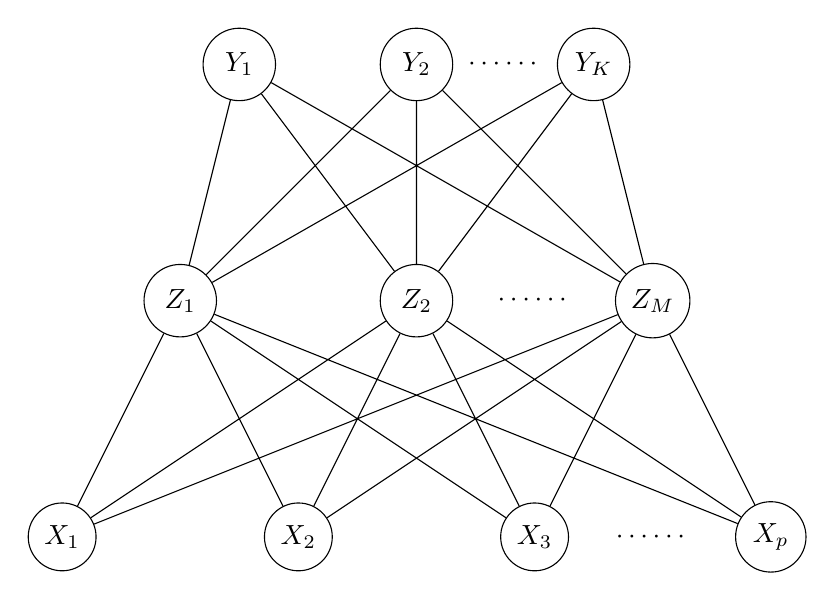
\begin{tikzpicture}[scale=1.5]
%\tikzstyle{every node}=[draw,shape=circle];
\draw (0,0) node [draw,shape=circle] (x1) {$X_1$};
\draw (2,0) node [draw,shape=circle] (x2) {$X_2$};
\draw (4,0) node [draw,shape=circle] (x3) {$X_3$};
\draw (5,0) node (xdots) {$\cdots\cdots$};
\draw (6,0) node [draw,shape=circle] (xp) {$X_p$};
\draw (1,2) node [draw,shape=circle,minimum height=0.92cm] (z1) {$Z_1$};
\draw (3,2) node [draw,shape=circle,minimum height=0.92cm] (z2) {$Z_2$};
\draw (4,2) node (zdots) {$\cdots\cdots$};
\draw (5,2) node [draw,shape=circle,minimum height=0.92cm] (zm) {$Z_M$};
\draw (1.5,4) node [draw,shape=circle,minimum height=0.92cm] (y1) {$Y_1$};
\draw (3,4) node [draw,shape=circle,minimum height=0.92cm] (y2) {$Y_2$};
\draw (3.75,4) node (ydots) {$\cdots\cdots$};
\draw (4.5,4) node [draw,shape=circle,minimum height=0.92cm] (yk) {$Y_K$};
\draw 
(x1) -- node[pos=0.1,above]{} node[pos=0.85,above]{} (z1)
(x1) -- node[pos=0.1,below]{} node[pos=0.85,below]{}(z2)
(x1) -- node[pos=0.1,above]{} node[pos=0.85,above]{} (zm)
(x2) -- node[pos=0.05,anchor=90]{} node[pos=0.85,below]{} (z1)
(x2) -- node[pos=0.1,below]{} node[pos=0.85,below]{} (z2)
(x2) -- node[pos=0.1,above]{} node[pos=0.85,above]{} (zm)
(x3) -- node[pos=0.1,above]{} node[pos=0.85,above]{} (z1)
(x3) -- node[pos=0.1,above]{} node[pos=0.85,above]{} (z2)
(x3) -- node[pos=0.1,above]{} node[pos=0.85,above]{} (zm)
(xp) -- node[pos=0.1,above]{} node[pos=0.85,above]{} (z1)
(xp) -- node[pos=0.1,above]{} node[pos=0.85,above]{} (z2)
(xp) -- node[pos=0.1,above]{} node[pos=0.85,above]{} (zm)
(z1) -- node[pos=0.1,above]{} node[pos=0.85,above]{} (y1)
(z1) -- node[pos=0.1,above]{} node[pos=0.85,above]{} (y2)
(z1) -- node[pos=0.1,above]{} node[pos=0.85,above]{} (yk)
(z2) -- node[pos=0.1,above]{} node[pos=0.85,above]{} (y1)
(z2) -- node[pos=0.1,above]{} node[pos=0.85,above]{} (y2)
(z2) -- node[pos=0.1,above]{} node[pos=0.85,above]{} (yk)
(zm) -- node[pos=0.1,above]{} node[pos=0.85,above]{} (y1)
(zm) -- node[pos=0.1,above]{} node[pos=0.85,above]{} (y2)
(zm) -- node[pos=0.1,above]{} node[pos=0.85,above]{} (yk)
;
\end{tikzpicture}
\]
\[
\begin{aligned} Z_{m} &=\sigma\left(\alpha_{0 m}+\alpha_{m}^{T} X\right), m=1, \ldots, M \\ T_{k} &=\beta_{0 k}+\beta_{k}^{T} Z, k=1, \ldots, K \\ f_{k}(X) &=g_{k}(T), k=1, \ldots, K 
\end{aligned}
\]


\end{document}
